\documentclass[12pt]{beamer}

\usetheme[sectionpage=none, subsectionpage=progressbar, progressbar=foot, numbering=fraction]{metropolis}

\makeatletter
\setlength{\metropolis@frametitle@padding}{1.6ex}% <- default 2.2 ex

\setbeamertemplate{footline}{%
  \begin{beamercolorbox}[wd=\textwidth, sep=1.5ex]{footline}% <- default 3ex
    \usebeamerfont{page number in head/foot}%
    \usebeamertemplate*{frame footer}
    \hfill%
    \usebeamertemplate*{frame numbering}
  \end{beamercolorbox}%
}
\makeatother

\AtBeginSubsection
{
  \begin{frame}{Where are we?}
    \tableofcontents[sectionstyle=show/shaded, subsectionstyle=show/shaded/hide]
  \end{frame}
}

\makeatletter
\setbeamertemplate{headline}{
  \begin{beamercolorbox}{upper separation line head}
  \end{beamercolorbox}
  \begin{beamercolorbox}{section in head/foot}
    \vskip2pt\insertsectionnavigationhorizontal{\paperwidth}{}{}\vskip2pt
  \end{beamercolorbox}
  \begin{beamercolorbox}{lower separation line head}
  \end{beamercolorbox}
}
\makeatother
\setbeamercolor{section in head/foot}{fg=normal text.bg, bg=structure.fg}

\setbeamertemplate{itemize items}[square]


\usepackage[UTF8]{ctex}
\usepackage{tabularx}


\title{Hacker Tools: \\Course Overview, Linux Install Fest, Virtual Machines}
\author{Julius Putra Tanu Setiaji}
\date{3 September 2019}

\begin{document}

\frame[plain]{\titlepage}

\section{Introduction}
\subsection{}

\begin{frame}{NUS Hackers}

  \begin{center}
    
\includegraphics[width=0.5\linewidth]{../NUSHackers}

    \url{http://nushackers.org}
  \end{center}

  \begin{center}
    \textbf{hacker}school

    Friday \textbf{Hacks}

    \textbf{Hack} \& Roll

    \textbf{Hacker} Tools
  \end{center}

\end{frame}

\begin{frame}{What is a Hacker?}
  A \textbf{hacker} is someone who strives to solve problems in elegant and ingenious ways.

  Hack as in hackathon.

  Read more at \url{https://www.nushackers.org/why/}

  Examples: Richard Stallman, Linus Torvalds, Jamie Zawinski, Steve Wozniak, Ken Thompson, Dennis Ritchie
\end{frame}

\begin{frame}{Hacker Tools}
  Inspired by \url{https://hacker-tools.github.io/}, organised by SIPB at MIT.

  Learn to make the most of the tools that hackers have been using for decades.

  In this class, we'll help you learn how to make the most of tools that productive programmers use.
\end{frame}

\begin{frame}{Course Overview}
  \begin{center}
    \begin{tabularx}{\textwidth}{l|l|X}
      \textbf{Week} & \textbf{Date \& Time, Venue} & \textbf{Topic}                      \\ \hline
      4             & 3/9/19 6.30pm, SR1           & Linux Install Fest, Virtual Machine \\ \hline
      5             & 10/9/19 6.30pm, SR10         & Shell \& Scripting                  \\ \hline
      6             & 17/9/19 7pm, SR1             & Command Line Environment            \\ \hline
      8             & 8/10/19 6.30pm, SR1          & Data Wrangling                      \\ \hline
      9             & 15/10/19 6.30pm, SR1         & Web Browsers \& Privacy             \\ \hline
      10            & 22/10/19 6pm, SR1            & Editors (vim \& emacs)              \\ \hline
      11            & 29/10/19 6.30pm, SR1         & OS Customisation                    \\ \hline
      12            & 5/11/19 6.30pm, SR1          & \LaTeX                              \\ \hline
    \end{tabularx}
  \end{center}
\end{frame}

\section{Linux}
\subsection{History}

\begin{frame}{What is Linux?}
  可以吃的吗?

  A Unix-like operating system kernel\footnote{The most fundamental part of an operating system -- it is a bridge between other software running on the computer and the hardware}.

  The most popular kernel in the world!

  Android, Chromebooks, most routers, most servers, supercomputers
\end{frame}

\begin{frame}{What is Unix?}
  A family of multi-tasking, multi-user operating system, first released in 1973.

  The first popular multi-user Windows was Windows 2000!

  Examples: macOS, iOS, SunOS/Solaris, BSD, AIX, HP-UX

  Most popular family of operating systems in the world!
\end{frame}

\begin{frame}{Most Popular OS Family in the world!}
  \begin{center}
    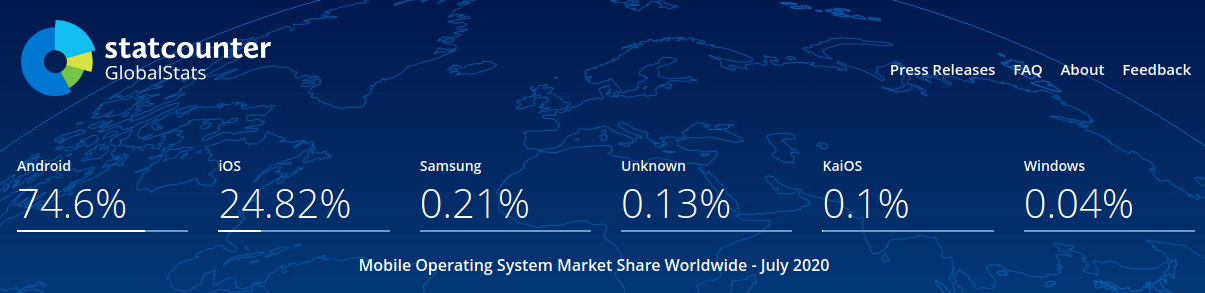
\includegraphics[width=0.75\linewidth]{phone-share}
  \end{center}

  \begin{columns}
    \begin{column}{0.5\linewidth}
      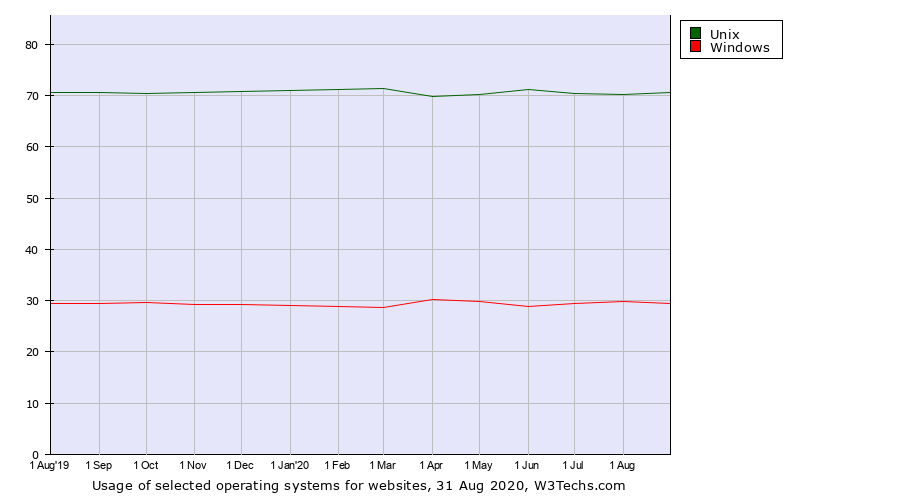
\includegraphics[width=\linewidth]{server}
    \end{column}
    \begin{column}{0.5\linewidth}
      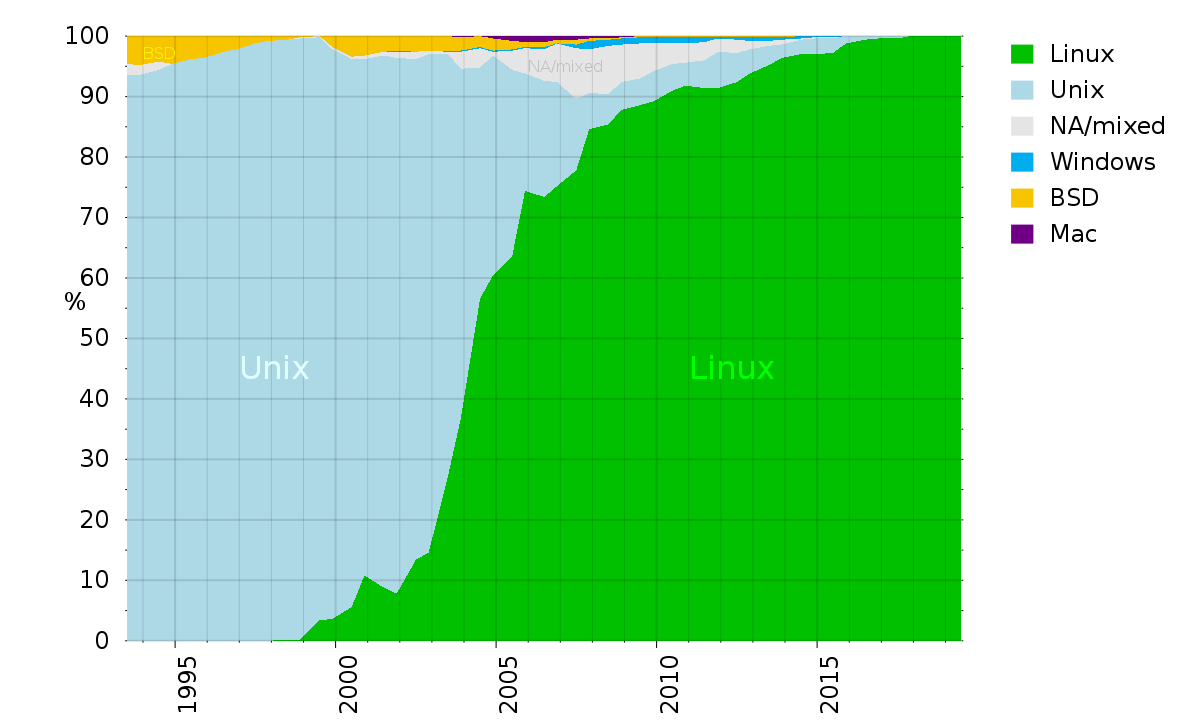
\includegraphics[width=\linewidth]{supercomputer}
    \end{column}
  \end{columns}
\end{frame}

\section{Virtual Machine}
\subsection{What? Why?}
\begin{frame}{What is a VM?}
  Virtual machines are simulated computer.

  You can configure a guest virtual machine with some operating system and configuration and use it without affecting your host environment.
\end{frame}

\begin{frame}{Why use a VM?}
  Experiment with operating systems, software, and configurations without risk.

  For running software that only runs on a certain operating system.

  For experimenting with potentially malicious software.
\end{frame}

\begin{frame}{Useful Features}
  \textbf{Isolation}

  Isolating the guest from the host, so you can use VMs to run buggy or untrusted software reasonably safely.

  \textbf{Snapshots}

  Snapshots capture the entire machine state.

  You can make changes to your machine, and then restore to an earlier state.

\end{frame}

\begin{frame}{Disadvantages}
  VMs are generally slower than running on bare metal.

  May be unsuitable for certain applications, e.g. Games, High Performance Computing.
\end{frame}

\begin{frame}{Examples}
  \begin{columns}
    \begin{column}{0.33\linewidth}
      \begin{center}
        
\includegraphics[width=0.8\linewidth]{parallels}
      \end{center}
    \end{column}
    \begin{column}{0.33\linewidth}
      
\includegraphics[width=\linewidth]{hyperv}
    \end{column}
    \begin{column}{0.33\linewidth}
      
\includegraphics[width=\linewidth]{vmware}
    \end{column}
  \end{columns}
  \begin{columns}
    \begin{column}{0.5\linewidth}
      
\includegraphics[width=\linewidth]{qemu}
    \end{column}
    \begin{column}{0.5\linewidth}
      \begin{center}
        
\includegraphics[width=0.7\linewidth]{virtualbox}
      \end{center}
    \end{column}
  \end{columns}
\end{frame}

\subsection{Installing}
\begin{frame}{Why VirtualBox?}
  
\includegraphics[width=0.7\linewidth]{virtualbox}

  We are going to use VirtualBox, because:
  \begin{itemize}
    \item It is FOSS (Free Open Source Software)
    \item It has a GUI (Graphical User Interface)
    \item It is cross-platform
  \end{itemize}
\end{frame}

\section{Conclusion}
\subsection{}
\begin{frame}
  \frametitle{Talk to us!}
  \begin{itemize}
    \item \textbf{Feedback form}: \url{https://is.gd/hs2019_hackertools_1}
    \item \textbf{Upcoming hackerschool}:
          \begin{itemize}
            \item Hackertools Part Two
          \end{itemize}
  \end{itemize}
\end{frame}

\end{document}
